\label{sec:tcomm}
In addition to the compute to I/O ratio discussed in Section \ref{sec:bound} we can define another performance parameter called the compute to communication ratio $t_{\text{comp}}/t_{\text{comm}}$.
In Section \ref{sec:I/O} we overcame the I/O effect by splitting the trajectory but scaling remained far from ideal when MPI communication was used (instead of  Global Arrays).
The task remained communication bound (Figure \ref{fig:MPIwithIO-split}), i.e, 
\begin{gather*}
  \frac{t_{\text{comp}}}{t_{\text{comm}}} \ll 1.
\end{gather*}

Figure \ref{fig:tcom_tcomm_effect} shows the relationship of performance with \tcomp/\tcomm ratio.
When the \tcomp/\tcomm ratio is higher, performance is better even if communication time is larger (Figure \ref{fig:tcomp_tcomm_ratio} and Figure \ref{fig:S2_tcomp_tIO_effect}).
Although there were stragglers due to communication their effect on performance remained modest because the overall performance was dominated by the compute load. 
Evidently, if overall performance is dominated by a component such as compute that scales well then  performance problems with components such as communication will be masked and overall acceptable performance can still be achieved.

\obnote{I am not sure what the point of the following is. Add values to quantify large/small? Correlate ratio with efficiency in graphs.}
Communication is usually not problematic within one node because of the shared memory environment.
As a result, communication time is not an issue even if the compute to communication ratio is small (Figure \ref{fig:tcomp_tcomm_ratio}, 1-24 cores represent a single compute node on \emph{SDSC Comet}).
However, beyond a single node, communication overhead becomes a bottleneck and effect of \tcomp/\tcomm becomes very important (Figure \ref{fig:tcomp_tcomm_ratio}, 24-72 cores represent multiple compute nodes on \emph{SDSC Comet}).

\begin{figure}[ht!]
\centering
\begin{subfigure}{.4\textwidth}
  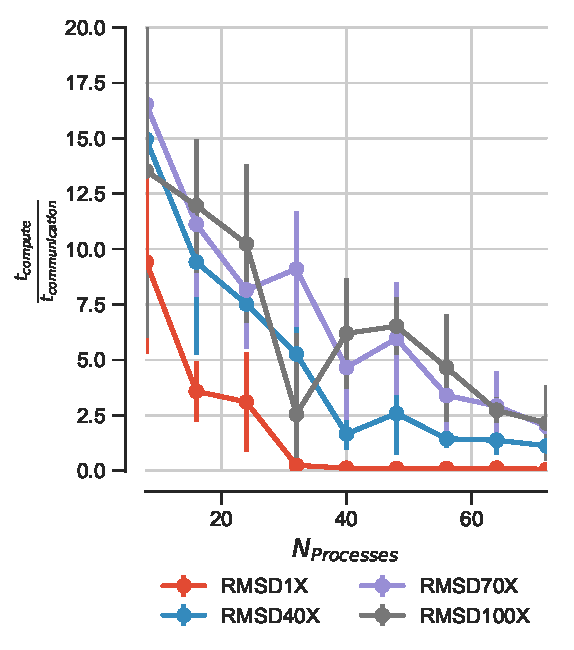
\includegraphics[width=\linewidth]{figures/Compute_to_comm_ratio_on_performance_v17.pdf}
  \captionsetup{format=hang}
\caption{Compute to communication ratio}
\label{fig:tcomp_tcomm_ratio}
\end{subfigure}
\hfill
\begin{subfigure}{.4\textwidth}
  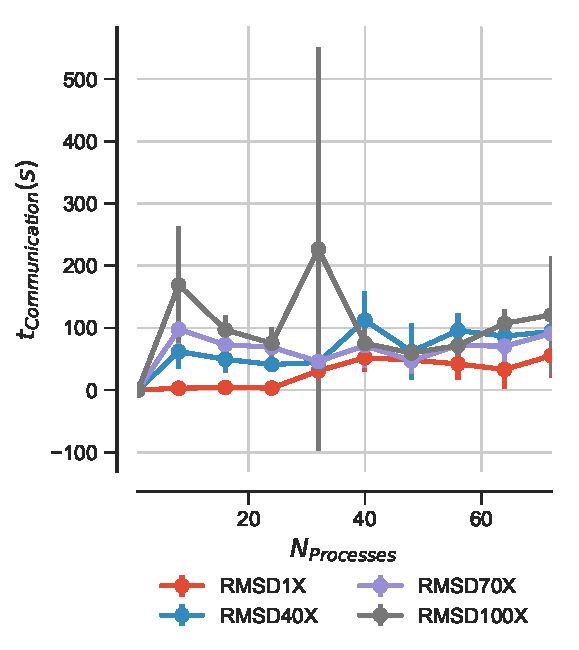
\includegraphics[width=\linewidth]{figures/comm_comparison_different_RMSD_overload.pdf}
  \caption{Communication time}
  \label{fig:MPItottime-chain-reader}
\end{subfigure}
\caption{(a) Change in compute to communication ratio with number of processes for different RMSD workload on SDSC Comet. 
(b) Comparison of communication time for different RMSD workload on SDSC Comet.
Five repeats were performed to collect statistics and error bars show standard deviation with respect to mean.}
\label{fig:tcom_tcomm_effect}
\end{figure}

%%% Local Variables:
%%% mode: latex
%%% TeX-master: t
%%% End:
